The Component Diagram shown below describes the logical components of the system we are to develop, from a very high-level description on to a more detailed one. This diagram does not take into account the deployment phase, hence it doesn't describe the logical layer of the system in terms of the physical tiers where it is deployed. It also does not show the interfaces between the logical layer and the end users or the database, for simplicity and readability. 


	\subsubsection{High level components}
		\paragraph{} We shall show below the high level view of the logical components of the system and their interactions. Following the UML 1 notation, the dashed arrows represent dependencies between components, with the tail end component depending on the point end component (e.g. if \textit{A $\rightarrow$ B}, then A \textit{depends on} B). 

		
		\begin{figure}[h]
			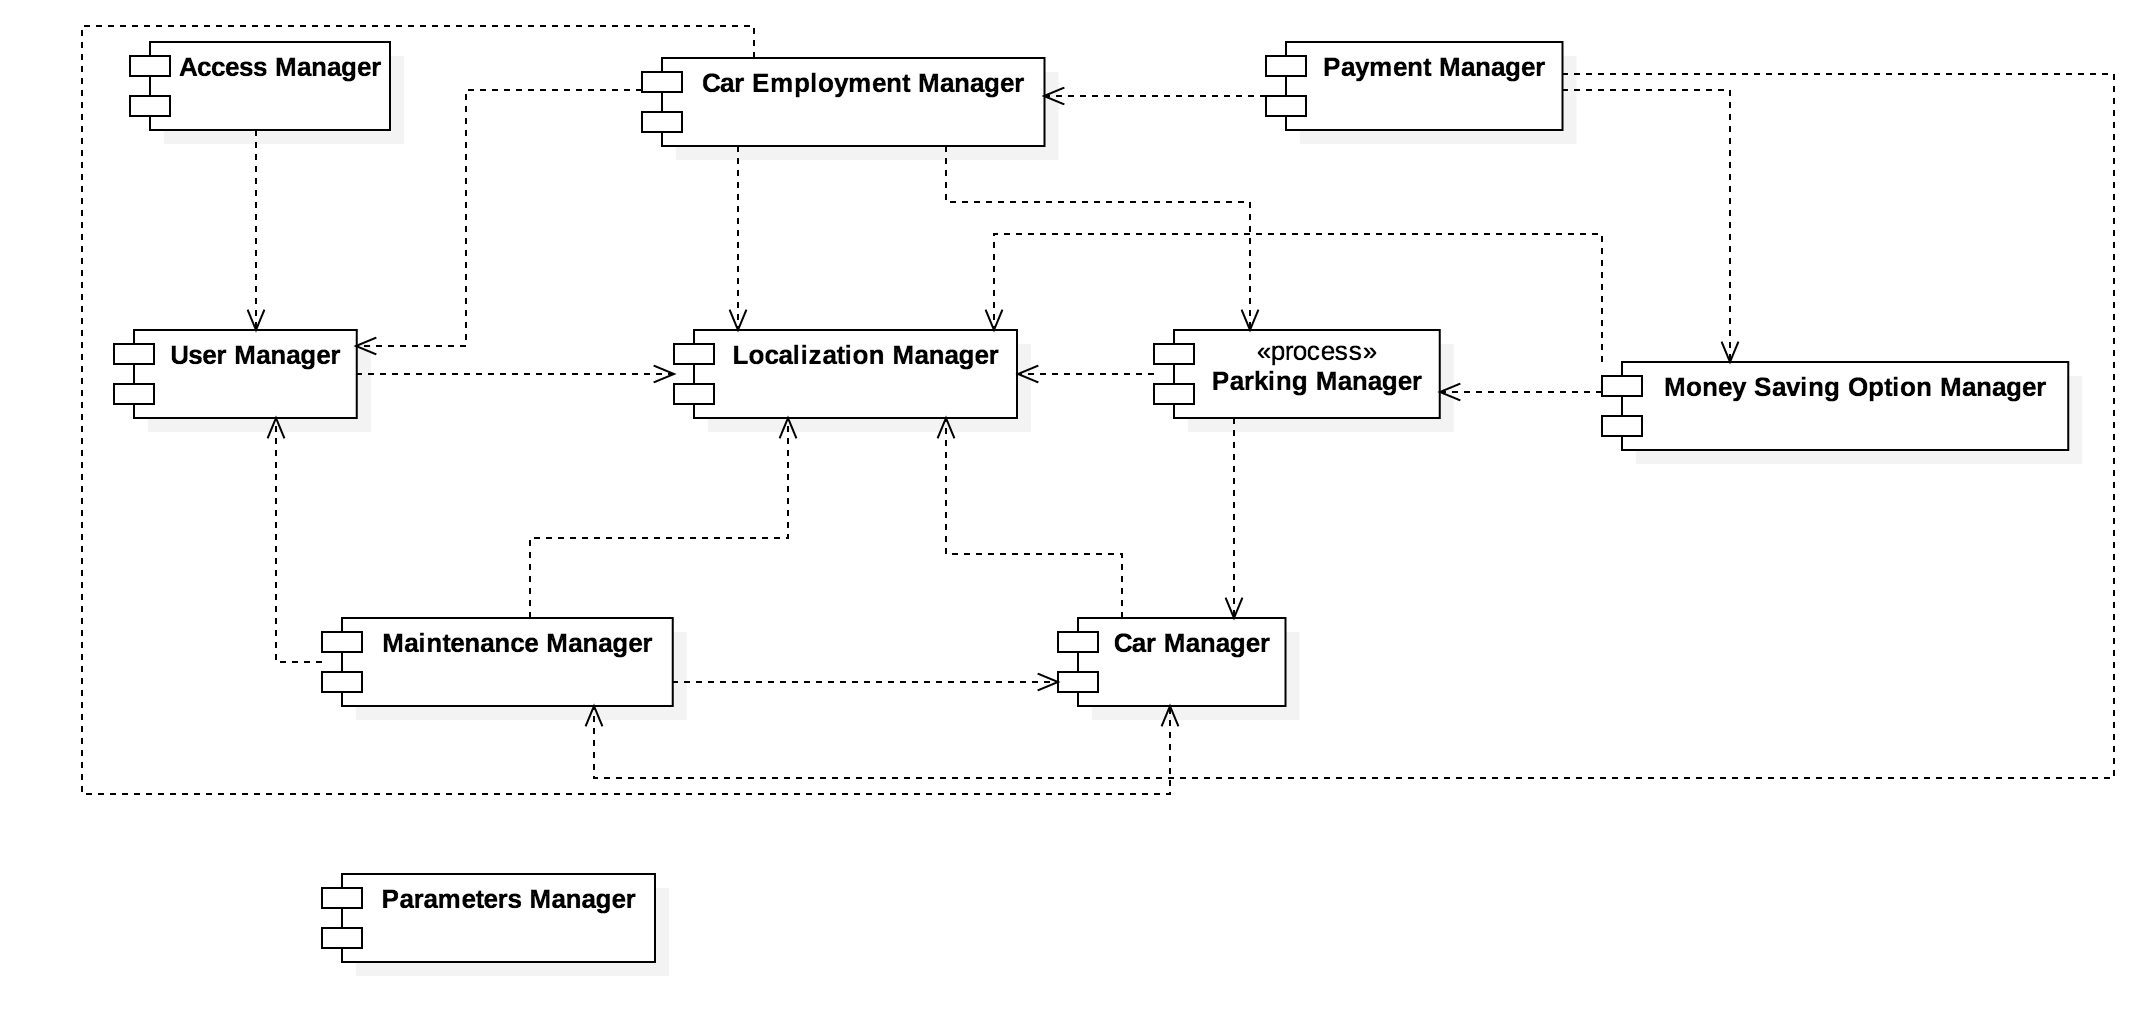
\includegraphics[scale=0.26, center]{img/component_diagrams/01_high_level_component_view.png}
			\caption{High level view}
		\end{figure}
\FloatBarrier


	\subsubsection{Component view}
	
	%\paragraph{Access Manager}
	\subsubsection*{Access Manager}
		
		
			
			
		\paragraph{}The Access Manager deals with the first interactions of a user or a guest with the system at the beginning of each session. Every further interaction with the system requires either a log in or the registration, both of which are managed by independent processes. The login interfaces with the User Handler to verify the validity of the login information and to allow the authenticated user to continue employing the system. Both processes also interface with the database.

		\begin{figure}[h]
				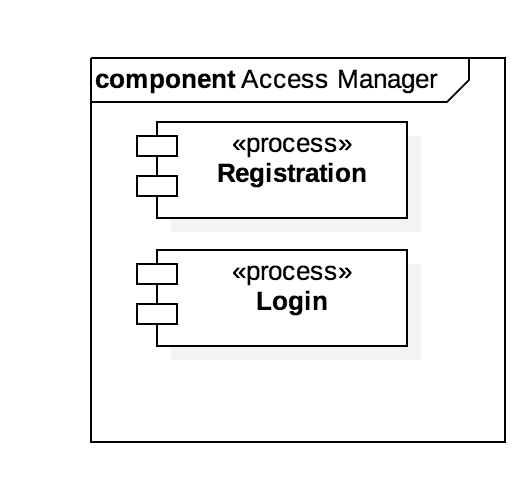
\includegraphics[scale=0.4, center]{img/component_diagrams/02_access_manager.png}
				\caption{Component Access Manager}
			\end{figure}
		
\FloatBarrier		
		
		\subsubsection*{User Manager}
		
		
		
		
		\paragraph{} The User Manager manages all interaction that a registered user has with the rest of the system. The User Handler functions as an interface component between the user themselves and the system, and to be associated with a user needs to be linked to the Profile Manager. This latter component interfaces with the DBMS and controls the validity of all data in the user's profile and its changes; the exception to this is the driving license data, that is checked by the License Manager since it's a particularly critical piece of information. The Profile Manager also depends on the License Manager in that every time the user tries to reserve a car the Profile Manager asks the License Manager for the validity of the user's license. 
		\begin{figure}[h]
			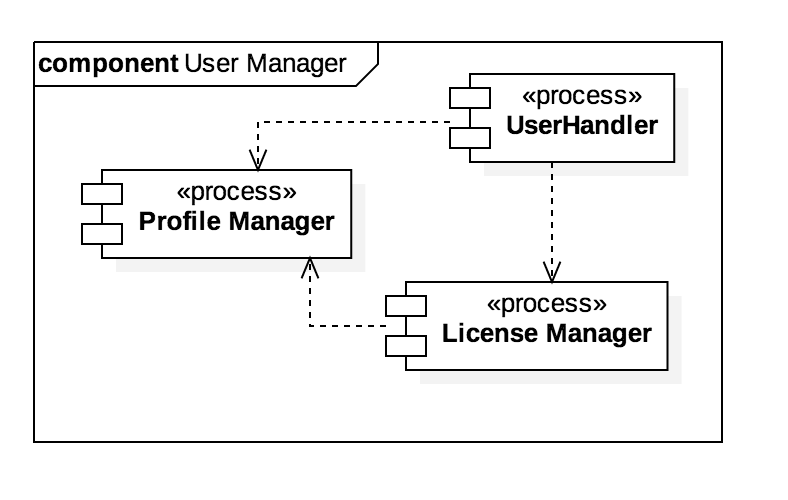
\includegraphics[scale=0.4, center]{img/component_diagrams/03_user_manager.png}
			\caption{Component User Manager}
		\end{figure}	
\FloatBarrier

		
		
		\subsubsection*{Car Employment Manager}
		
			
			
		\paragraph{} The Car Employment Manager is one of the most important component of the system in terms of its core functionalities. It's composed of three processes: the first one, the Reservation Handler, has the task of dealing with reservations from a user and for an individual car. It blocks all other possible operations to that car until the user starts using it or the reservation expires. To keep track of the time, the Reservation Handler needs to interface with the Time Manager. This process is tasked with keeping track of the time periods necessary for the services to be offered: the expiration time for a reservation, the duration of a ride, the time window after a ride has finished. 
		The Ride Handler on the other hand depends on the Reservation Handler in that a car can be used only after a reservation. The Ride Handler is associated to a particular car and a particular user. It depends on the Time Manager to keep track of the duration of the ride. 
		\begin{figure}[h]
			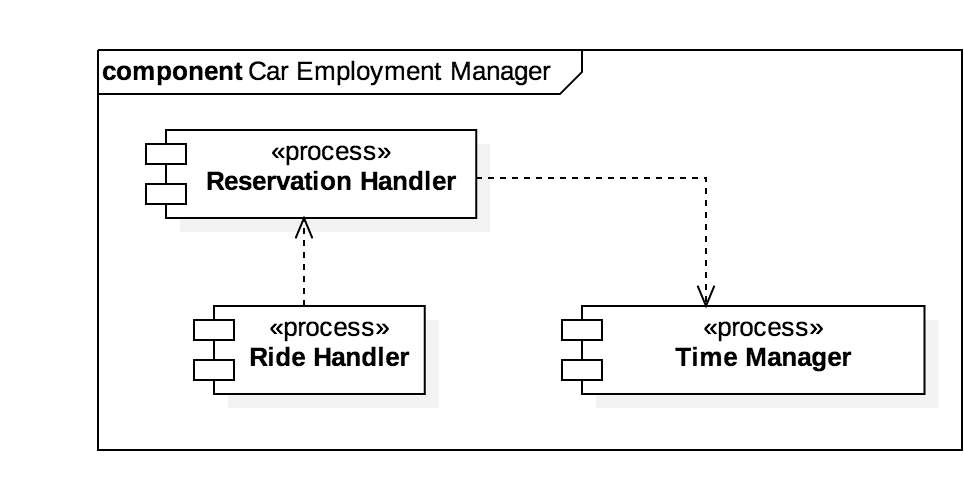
\includegraphics[scale=0.4, center]{img/component_diagrams/04_car_employment_manager.png} %TODO modify the image, a dependency is missing
			\caption{Component Car Employment Manager}
		\end{figure}	
\FloatBarrier

		
		
		\subsubsection*{Localization Manager}
		
		
			
		\paragraph{} The Localization Manager handles all the localization issues of the system. Its three components, the User Location Handler, the Car Location Handler and the Operator Location Handler (that track, respectively, users, cars and operators) all work independently from each other and interface with the respective handlers from other components. The Localization Manager also interfaces with the external Map Services Provider, that provides the information for the localization.
		\begin{figure}[h]
			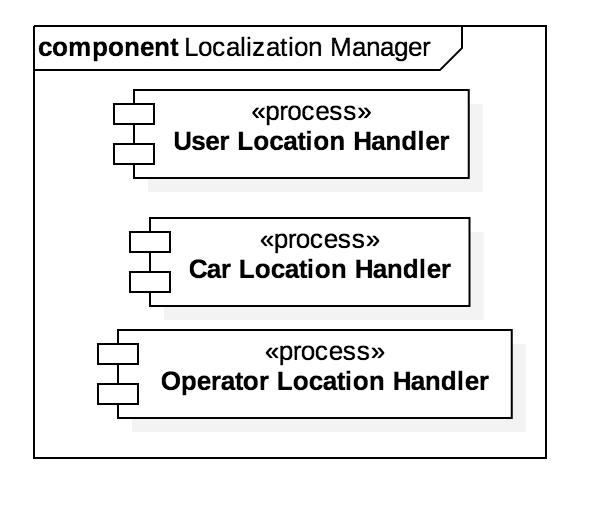
\includegraphics[scale=0.4, center]{img/component_diagrams/05_localization_manager.png}
			\caption{Component Localization Manager}
		\end{figure}	
\FloatBarrier		
		
		
		\subsubsection*{Maintenance Manager}
		
		
		\paragraph{} The Maintenance Manager deals with emergencies and daily maintenance of the cars. For this purpose, it has an interface with the operators, the Operator Handler; the operators are dispatched by the admins and are associated to some emergency report. The Dispatcher Manager handles the availability and the tasks associated with each operator; the Emergency Report Handler on the other hand manages the emergency reports, associating them with a user, a car and an operator, and keeping track of their status thanks to the Report Status Handler.
		\begin{figure}[h]
			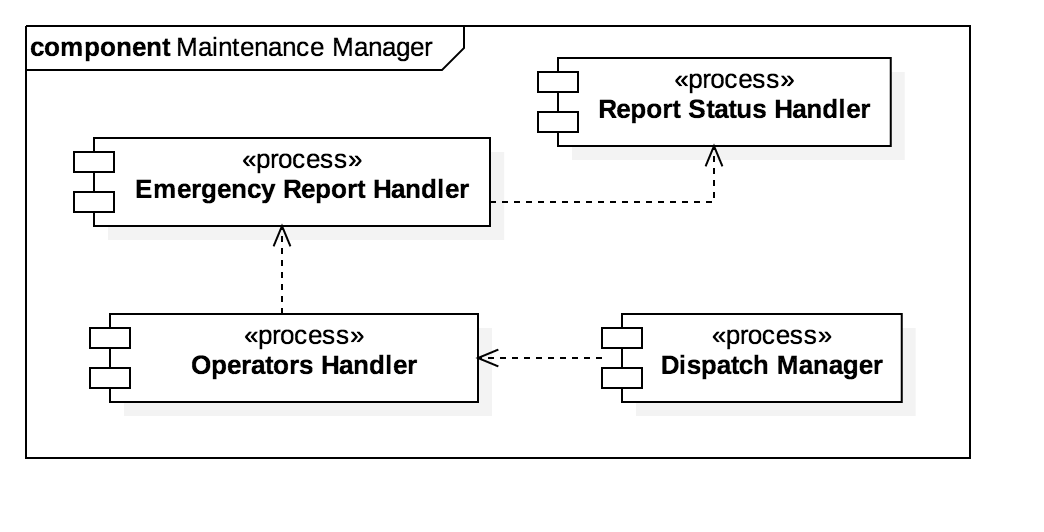
\includegraphics[scale=0.4, center]{img/component_diagrams/06_maintenance_manager.png}
			\caption{Component Maintenance Manager}
		\end{figure}	
		

\FloatBarrier		
		
		
		
		\subsubsection*{Backend Manager}
			
			
		\paragraph{} The Backend Manager oversees all operations entrusted to the administrators. The Admin Handler is the interface between the admins and the system, and keeps track of each administrator's activities and identification. The Parameters Manager deals with all changes done to the parameters of the system (their validity within fixed boundaries, their actual deployment); the Admin Handler depends on it since every change to the parameters is done by an admin. %FIXIT actual deployment??
		\begin{figure}[h]
				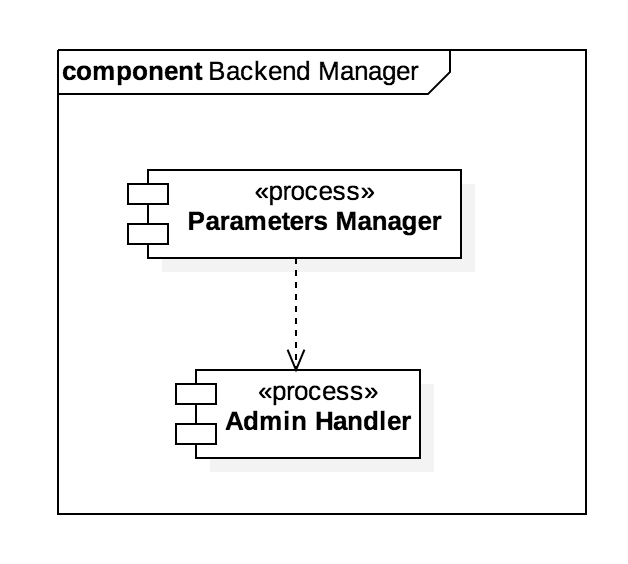
\includegraphics[scale=0.4, center]{img/component_diagrams/11_backend_manager.png}
				\caption{Component Backend Manager}
			\end{figure}
\FloatBarrier
	
		
		
		
		\subsubsection*{Car Manager}
			
		
		\paragraph{} The Car Manager interfaces the car with the rest of the system. The Sensors Manager gathers and parses the raw signals provided by all the sensors in the car. It also is the direct line of communication between the car and the Car Handler. The Car Handler interprets the information provided by the Sensors Manager and acts upon it, notifying other components or giving commands to the sensors.
		 \begin{figure}[h]
				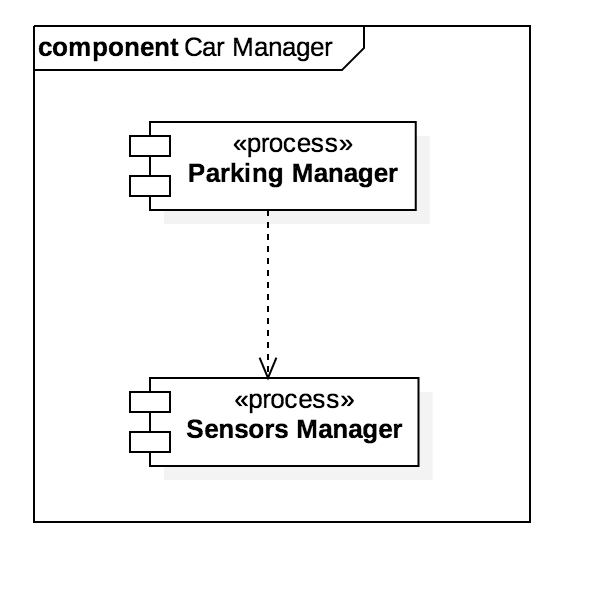
\includegraphics[scale=0.4, center]{img/component_diagrams/07_car_manager.png}
				\caption{Component Car Manager}
			\end{figure}
\FloatBarrier
		
		
		
		
		\subsubsection*{Payment Manager}
			
			
		\paragraph{} Through the Payment Manager, the system keeps track of the fare of each ride and the extraordinary fees (i.e. the fines), the discounts and the sanctions to charge the user. The Payment Handler is arguably the most important process since it's the one that is tasked with keeping track of the total cost for a ride. To do that, it needs to interface with the Ride Handler, and also with the Discounts and Sanctions Handler, to be able to consider them in its calculations. The Exceptional Payment Handler manages the exceptional fees, such as fines for expired reservations or for damages to the car. All of them are needed by the Invoice Manager, that takes the final charge from them and notifies the external Payment Services Provider, such that it may invoice the user of their charges.
		\begin{figure}[h]
				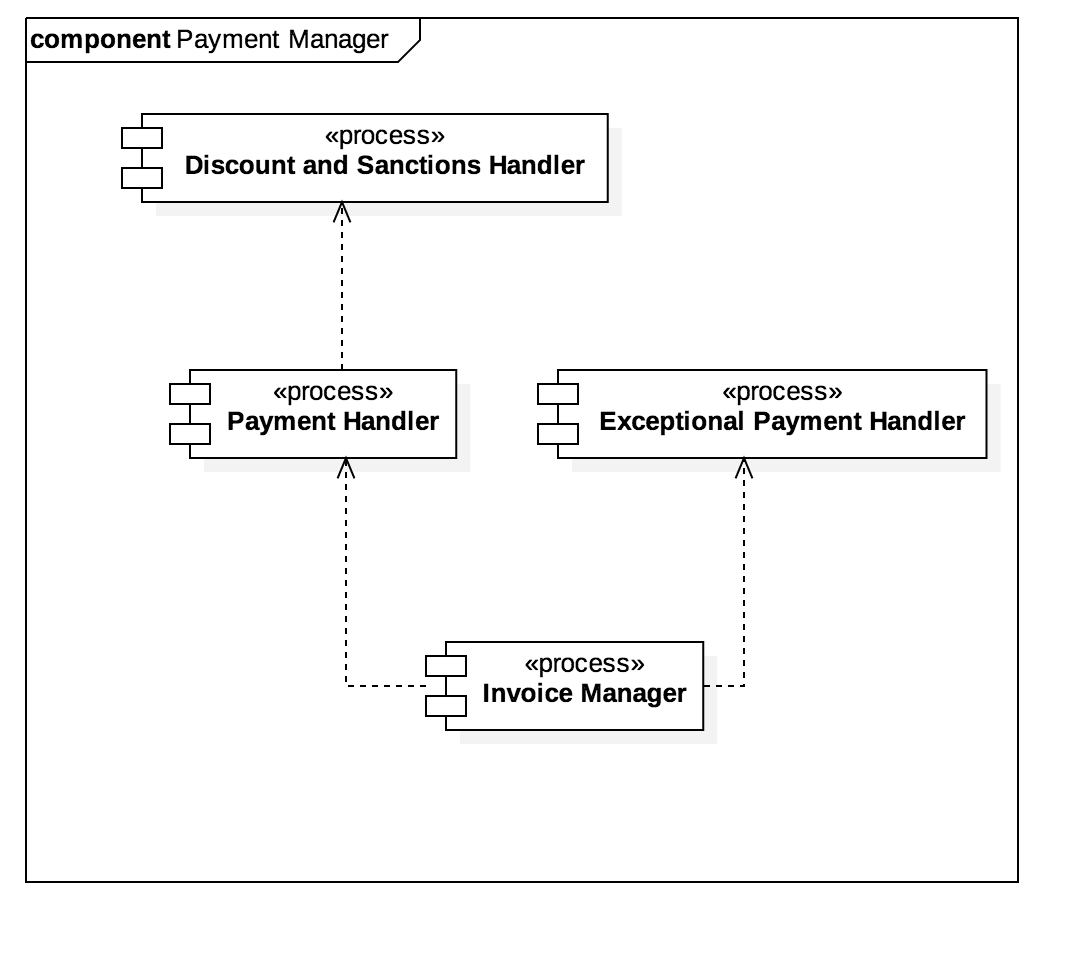
\includegraphics[scale=0.4, center]{img/component_diagrams/08_payment_manager.png}
				\caption{Component Payment Manager}
			\end{figure}
\FloatBarrier	
		
		
		
		\subsubsection*{Money Saving Option Manager}
			
		
		\paragraph{} We decided to dedicate an entire component for the sole purpose of managing the Money Saving Option (MSO), because of its complexity. The Discounts and Sanctions Handler also depends on this component to provide the information on whether to apply the relative discount or not. It has two processes, which are the Parking Distribution Handler and the MSO Handler. The Parking Distribution Handler takes the brunt of the computing complexity since its task is to calculate the optimal distribution of cars with an heuristic algorithm. On the other hand, the MSO Handler gets the necessary information from the Parking Distribution Handler and decides which Parking Area to notify the user given the destination of the ride.
		%FIXIT TMI?
		\begin{figure}[h]
				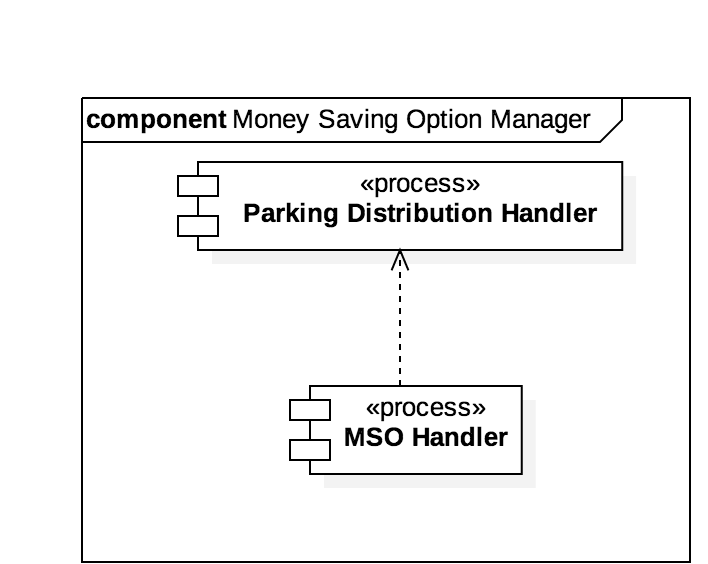
\includegraphics[scale=0.4, center]{img/component_diagrams/09_money_saving_option_manager.png}
				\caption{Component Money Saving Option Manager}
			\end{figure}
\FloatBarrier		
		
		\subsubsection*{Parking Manager}
		
			%FIXIT no image? do we need it?
		
		\paragraph{} The Parking Manager keeps tabs on where (and if) a car is parked, and for how long. Thanks to the Car Location Manager and the Car Sensors, it locates cars and decides whether they are parked inside a Safe Area or not; it also depends on the Time Manager to calculate the window of time after the end of a ride when a user is still allowed to plug the car into the power grid or open it.
		%FIXIT change direction of arrow between time manager and parking manager?
\FloatBarrier

	\subsubsection{Complete component view}
	
	The following figure shows the complete component diagram for the system, with all the dependencies as shown. 
	
		\begin{sidewaysfigure}
			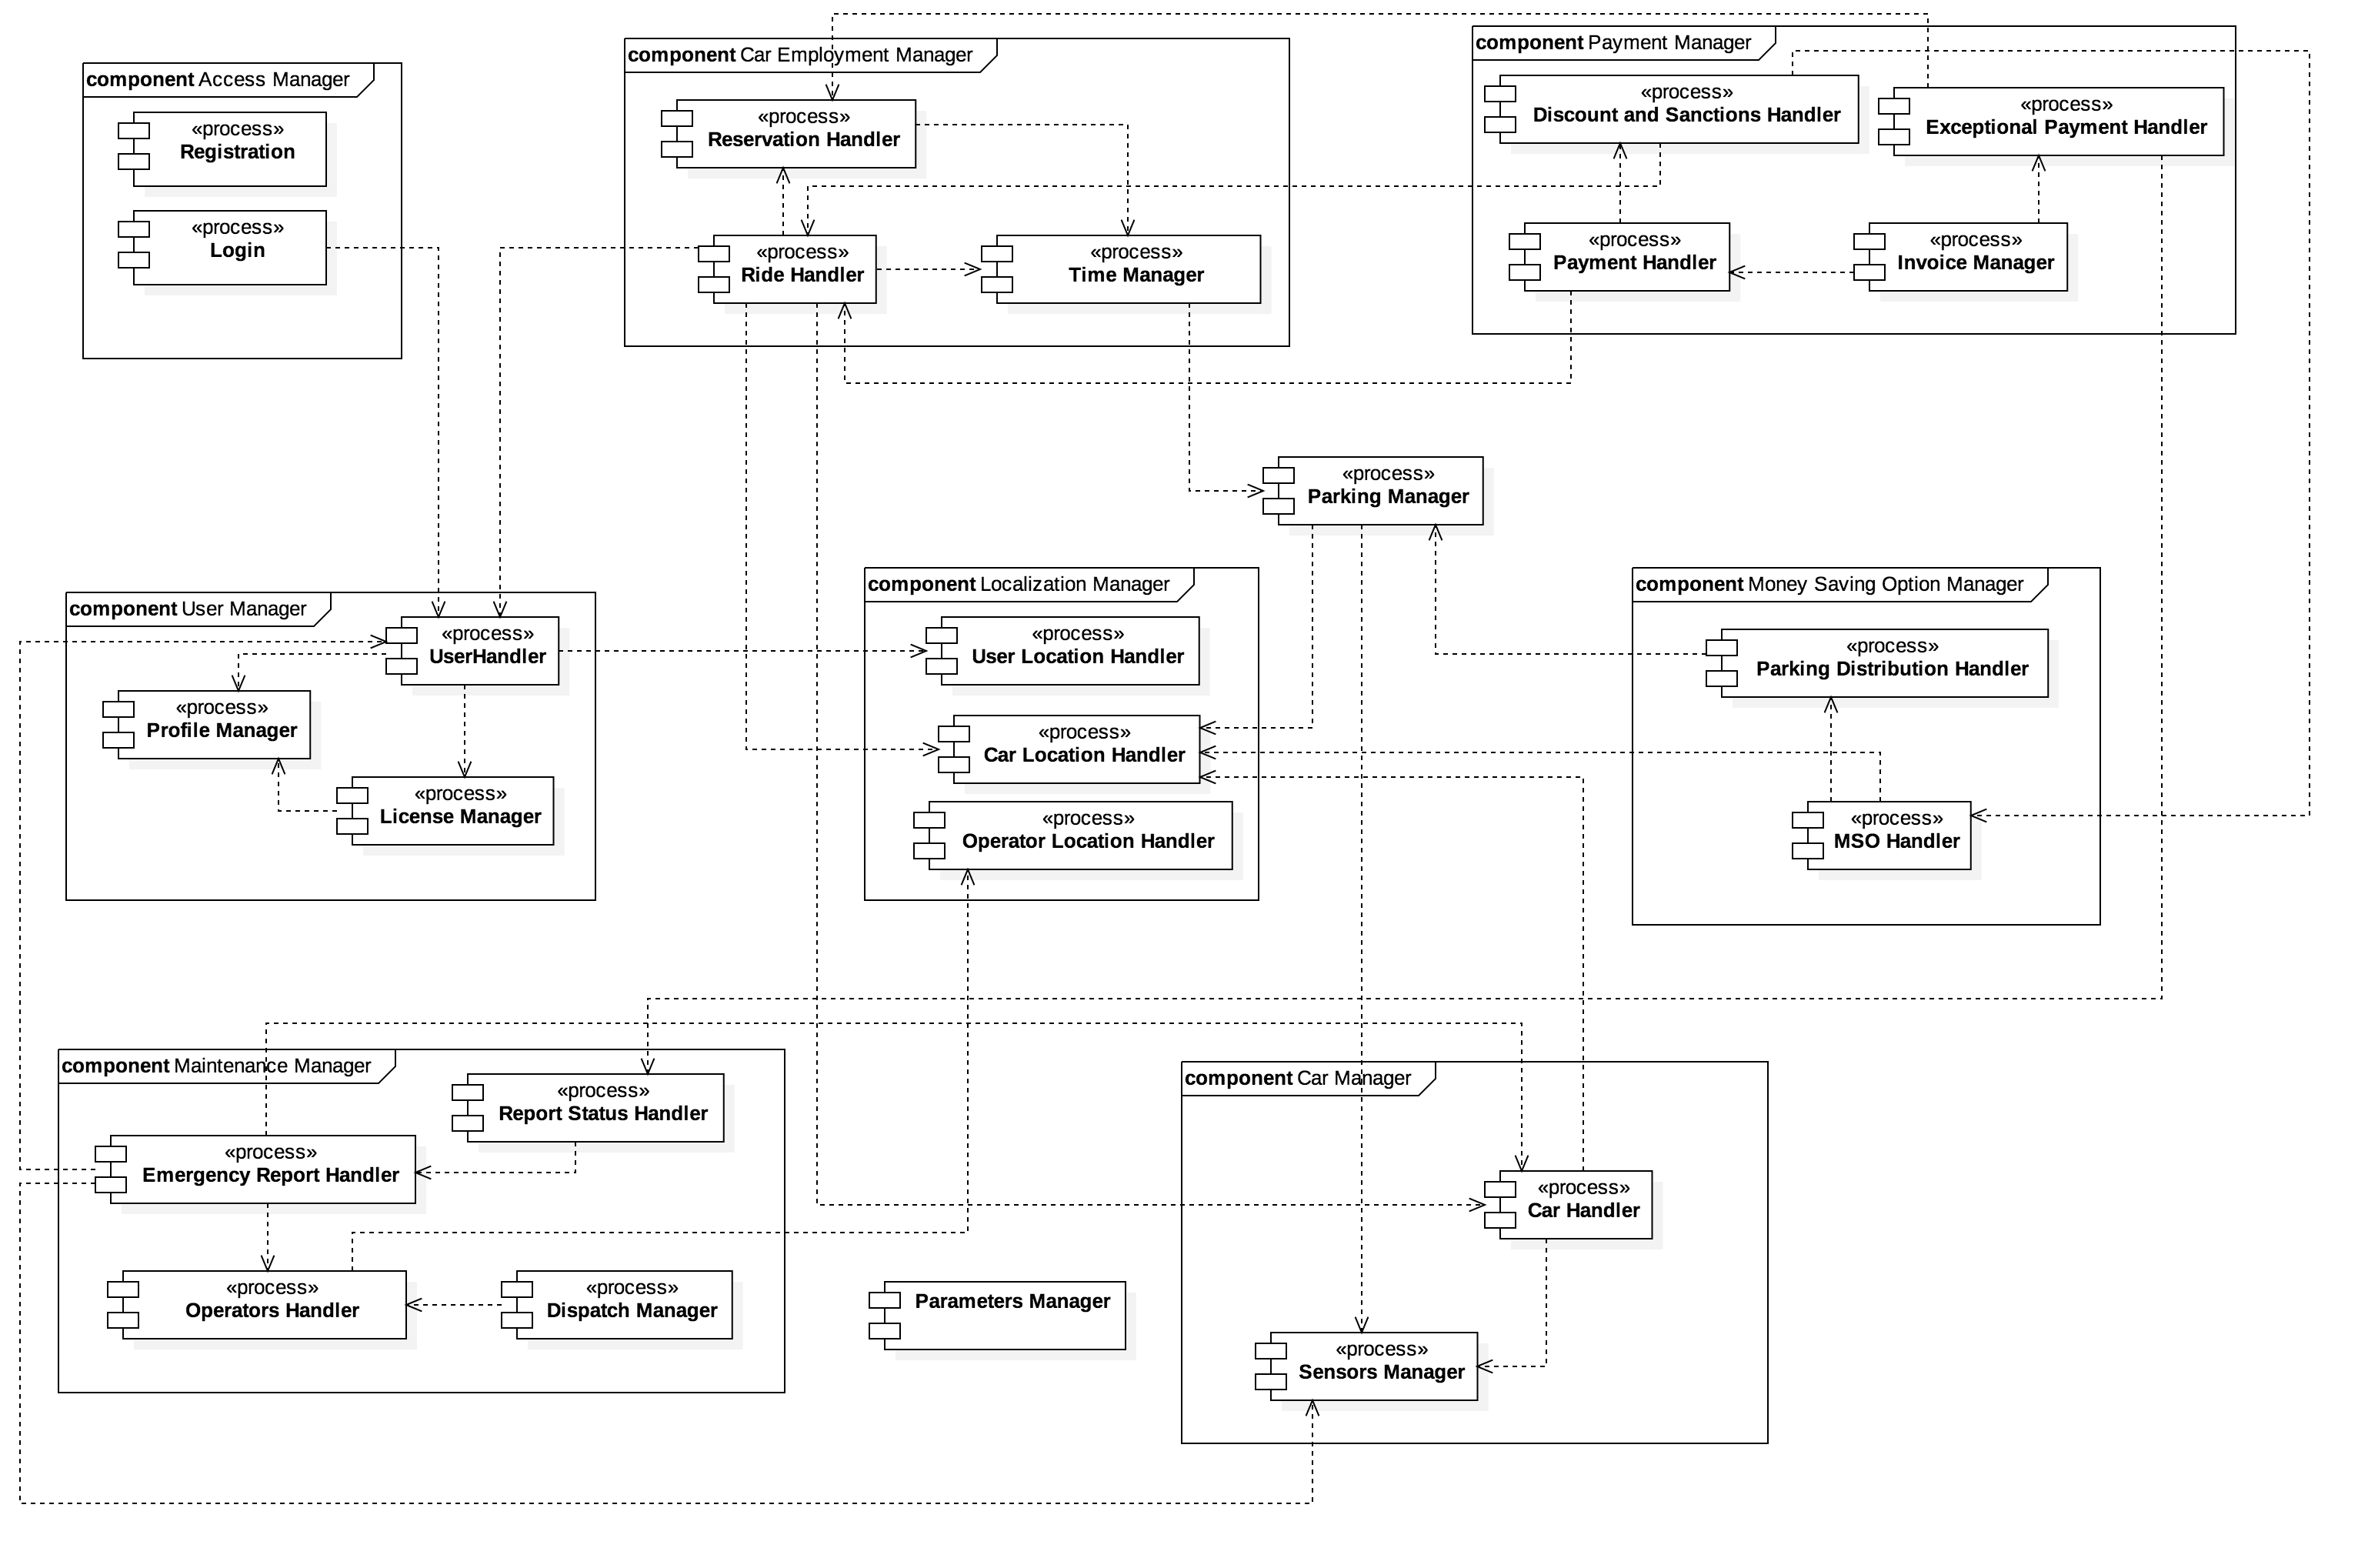
\includegraphics[width=\hsize, center]{img/component_diagrams/10_complete_component_view.png}
			\caption{Complete Component View}
		\end{sidewaysfigure}
			
\FloatBarrier
